\documentclass[aps,prl,reprint,longbibliography]{revtex4-1}

\usepackage{graphicx}
\graphicspath{{figures/}}
\usepackage{siunitx}
\usepackage{amsmath}

\renewcommand{\vec}[1]{\mathbf{#1}}

\begin{document}

\title{Projecting non-diffracting waves with intermediate-plane
holography}

\author{Argha Mondal}
\author{Aaron Yevick}
\author{Lauren C. Blackburn}
\author{Nikitas Kanellakopoulos}
\author{David G. Grier}

\affiliation{Department of Physics and Center for Soft Matter Research,
New York University, New York, NY 10003}

\begin{abstract}
  We introduce an approach to phase-only holography that substantially
  improves the ability of holographic trapping systems to project
  propagation-invariant modes of light.
  This technique is particularly well suited for projecting
  accelerating modes and long-range tractor beams.
\end{abstract}

\maketitle

Structuring laser beams with computer-generated holograms
has revolutionized optical micromanipulation \cite{grier03} and
optical communication \cite{gibson04,bozinovic13,willner15}.
Using holograms to project propagation-invariant modes of light,
for example, has led to the remarkable
discovery that some non-diffracting modes
can act as tractor beams, pulling illuminated objects
upstream rather than trapping them or pushing them downstream
\cite{marston06,lee10}.
Applications of tractor beams and other exotic light modes have
been hampered by the poor diffraction efficiency of the
holograms used to project them, which can be less
than \num{e-3} \cite{ruffner12a,ruffner14}.
To address this problem, we introduce intermediate-plane
holography, a technique that relaxes constraints typically
employed in the holographic trapping technique \cite{grier03}, to improve
both diffraction efficiency and mode purity.
We illustrate these capabilities by projecting
Bessel beams, which constitute 
the natural basis for propagation-invariant modes \cite{durnin87,durnin87a}.
We then use these techniques to project meter-long
optical conveyors \cite{cizmar05,ruffner12a,ruffner14}
and solenoid beams \cite{lee10,yevick16}, 
which are tractor-beam modes composed of superpositions of Bessel
beams.
These experiments demonstrate a \num{400}-fold improvement in 
diffraction efficiency relative to the standard holographic optical
trapping technique, and a
\num{1000}-fold increase in non-diffracting range.

Holograms intended for optical micromanipulation typically
are designed to modify the phase profile of an incident laser beam,
but not the amplitude.
The phase-only hologram then propagates to a converging
lens that transforms it into the intended mode.
Scalar diffraction theory approximates this transformation
as a Fourier transform \cite{goodman05}.
Difficulties are encountered when the Fourier transform of
the desired mode features amplitude variations
that can not be encoded naturally in a phase-only diffractive optical element.

For example, the ideal complex-valued hologram encoding 
an $m$-th order Bessel beam takes the form of an infinitesimally
fine ring,
\begin{equation}
  \label{eq:besselhologram}
  E_{\alpha,m}(\vec{r},0)
  =
  \delta(r - R_\alpha) \, e^{i m\theta},
\end{equation}
whose radius, $R_\alpha = f \, \tan\alpha$,
depends on the focal length of the projecting lens, $f$,
and the desired convergence angle of the Bessel
beam, $\alpha$.
Equation~\eqref{eq:besselhologram} expresses the
scalar field in terms of the two-dimensional
polar coordinates, $\vec{r} = (r,\theta)$, in the plane $z = 0$.
More generally, $E_{\alpha,m}(\vec{r},z)$ describes transverse profile
of the same field at axial position $z$.

The ideal ring hologram consists of an amplitude mask, shown
schematically in
Fig.~\ref{fig:intermediate}(a),
that only allows light to pass through the thin annulus at radius
$R_\alpha$, and a phase mask that imposes a helical pitch on the
transmitted wavefronts.
The same effect can be achieved with a
phase-only hologram,
\begin{equation}
  \label{eq:idealbesselhologram}
  \varphi_{\alpha,m}(\vec{r})
  =
  \begin{cases}
    m \theta \bmod 2 \pi, & r = R_\alpha \\
    \varphi_0(\vec{r}), & \text{otherwise}
  \end{cases}
\end{equation}
where $\varphi_0(\vec{r})$ is an undetermined
phase function that diverts light away from the
optical axis \cite{roichman06}.

Equation~\eqref{eq:idealbesselhologram}
poses two substantial problems for standard
holographic trapping implementations
of the kind represented in Fig.~\ref{fig:intermediate}(a).
In the first place, the delta-function
amplitude profile in the hologram plane cannot be encoded
faithfully on a pixellated diffractive optical element.
The bright ring in Fig.~\ref{fig:intermediate}(a) represents
the intensity,
$I(\vec{r},0) = \left\vert  E_{\alpha,0}(\vec{r},0)\right\vert^2$,
projected by an $m = 0$ ring hologram, treated as an
ideal amplitude mask.
The ring's finite thickness arises from the mask's
finite pixel size.
Rather than projecting a wave with a single value of $\alpha$,
this finite-thickness ring constitutes a superposition of
ring holograms that corresponds to a
superposition of Bessel beams with
a range of convergence angles, $\alpha$.
Interference among these superposed modes
causes periodic axial intensity variations,
and so limits the propagation-invariant
range of the superposition \cite{ruffner12a}.
In the second place, only a few pixels in
the hologram plane contribute to the intended Bessel beam.
The rest of the hologram's area is dedicated to the
phase function $\varphi_0(\vec{r})$ that diverts
extraneous light away from the desired mode.
Pixellated ring holograms thus suffer from a combination of
poor mode fidelity and extremely poor diffraction efficiency.

\begin{subequations}
\label{eq:intermediatebesselhologram}
Both deficiencies can be mitigated by considering
light's propagation from the hologram plane to the converging
lens.  The field at distance
$z$ along the optical axis may be estimated with the
Rayleigh-Sommerfeld diffraction integral \cite{born99},
\begin{equation}
  \label{eq:rayleighsommerfeld}
  E(\vec{r},z)
  =
  \int \tilde{E}(\vec{q},0) \tilde{H}_z(\vec{q}) e^{- i \vec{q} \cdot \vec{r}} \,
  d^2q ,
\end{equation}
where $\tilde{E}(\vec{q},0)$
is the two-dimensional Fourier transform of the field
$E(\vec{r},0)$ in the plane $z = 0$
and
\begin{equation}
  \label{eq:propagator}
  \tilde{H}_z(\vec{q}) 
  =
  e^{i z \sqrt{k^2 - q^2}}
\end{equation}
is the Fourier transform of the Rayleigh-Sommerfeld propagator
for light of wave number $k$ \cite{goodman05}.
\end{subequations}
Because the light diffracts as it propagates,
challenging amplitude variations in $E(\vec{r},0)$
can be substantially less pronounced in the intermediate plane
at axial position $z$.
This can be seen in the intermediate-plane intensity,
$I(\vec{r},z) = \left\vert E_{\alpha,0}(\vec{r},z) \right\vert^2$,
for the $m = 0$ mode in Fig.~\ref{fig:intermediate}(a).
A phase-only hologram designed for this plane therefore will have
much better diffraction efficiency than the ideal
hologram designed for $z = 0$.
Indeed, the location, $z$, of the intermediate plane
can be selected to maximize this benefit.
Improving diffraction efficiency naturally improves
mode fidelity by reducing the amount of light in
unwanted modes.
Performance may be even better than this observation
suggests because $E(\vec{r},z)$ is
computed from the ideal field, without compromise
for pixellation.

The phase-only intermediate-plane hologram associated with
$E(\vec{r},0)$ may be approximated by the phase, $\varphi(\vec{r},z)$,
of $E(\vec{r},z)$, ignoring amplitude variations.
The intermediate-plane phase for the $m = 0$ Bessel beam
is presented in Fig.~\ref{fig:intermediate}(b).
If necessary, some accommodation may be made for remaining
amplitude variations through any of the techniques
that have been developed for encoding complex-valued
fields on phase-only diffractive optical elements \cite{roichman06}.
In practice, this often is unnecessary, and the phase of the
computed intermediate-plane field often serves as a
mode-forming hologram with high diffraction efficiency.

The benefits of intermediate-plane holography come at
a cost.  Specifically, the diffractive optical element no
longer is located in the focal plane of the projecting
lens.  This requires modifying the optical layout of a typical
holographic trapping system.
For the particular case of reflective holograms,
space constraints may limit the range of $z$,
and thus the benefit of the technique.
In cases where large positive values of $z$ are 
physically inaccessible,
negative values may offer the same benefits while
affording sufficient space for practical implementation.

\begin{figure}[t!]
  \centering
  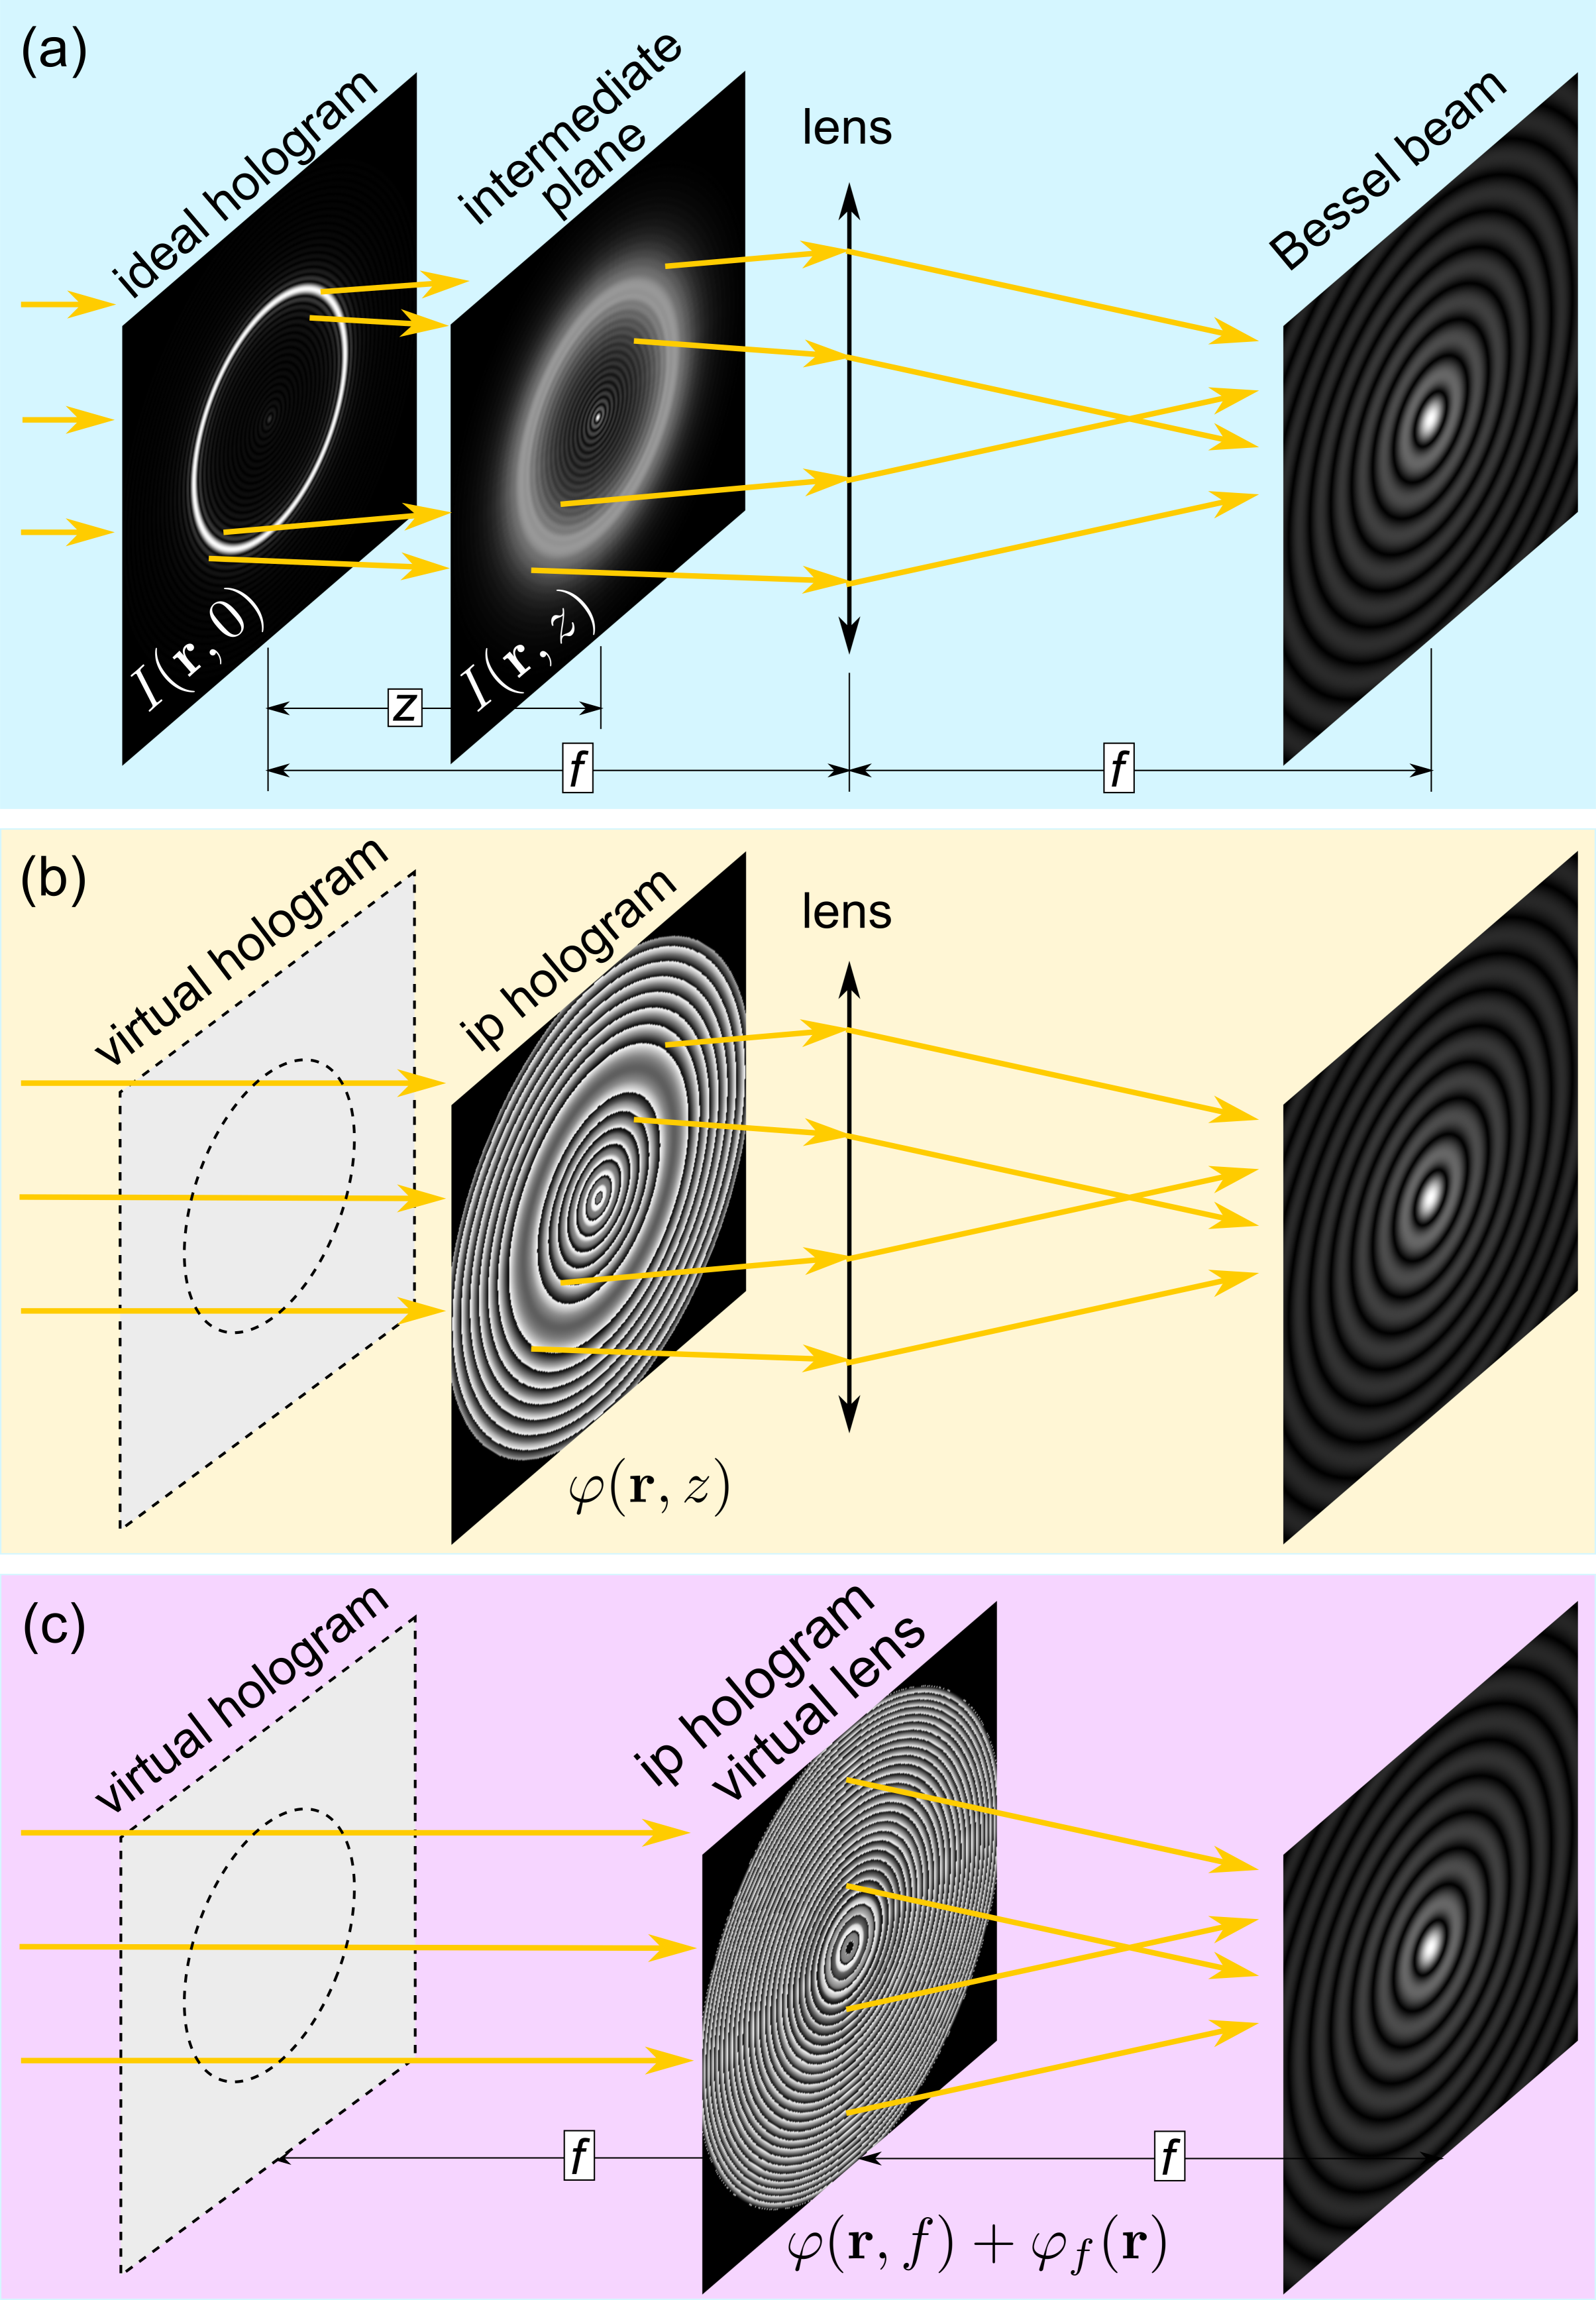
\includegraphics[width=\columnwidth]{intermediate2}
  \caption{Intermediate-plane holography. (a) Conventional
    holographic projection of a Bessel beam.  The field diffracted
    by a ring hologram propagates to a converging lens of
    focal length $f$ that
    projects it into the non-diffracting mode.
    (b) A phase-only hologram
    in an intermediate plane recreates the ring-hologram's
    wavefront structure at substantially higher diffraction efficiency.
    (c) Moving the intermediate plane to $z = f$ and incorporating
    the phase function for a converging lens of focal length $f$
    creates a mode converter that projects the Bessel beam directly.}
  \label{fig:intermediate}
\end{figure}

Setting $z = f$ addresses these geometric considerations
by placing the intermediate-plane hologram
in the same plane as the converging lens.
The associated parabolic phase profile,
\begin{equation}
  \label{eq:lensphase}
  \varphi_f(\vec{r}) = \frac{\pi r^2}{\lambda f}
  \bmod 2 \pi,
\end{equation}
can be integrated into the phase function
for the intermediate-plane hologram, 
\begin{equation}
  \label{eq:complete}
  \varphi(\vec{r}) 
  =
  \left[\varphi(\vec{r},f) +
  \varphi_f(\vec{r}) \right]
  \bmod 2 \pi, 
\end{equation}
thereby eliminating the need for
the physical lens altogether.
This mode of operation is presented in
Fig.~\ref{fig:intermediate}(c) and is the
approach we will adopt for experimental demonstrations.

%Unresolvably fine features in $E(\vec{r},0)$, 
%moreover, will be expanded by diffraction and so can
%be better represented on a pixelated diffractive optical
%element.

For the particular case of a Bessel beam,
the Fourier transform of the ideal ring hologram is
\begin{equation}
  \tilde{E}_{\alpha,m}(\vec{q},0)
  =
  J_m(qR_\alpha) \, e^{i m \theta}.
\end{equation}
Applying Eq.~\eqref{eq:intermediatebesselhologram}
then yields an expression for the field in the 
intermediate plane,
\begin{equation}
  \label{eq:radialintegral}
  E_{\alpha,m}(\vec{r},z)
  =
  e^{i m \theta}
  \int_0^k 
  q 
  J_m(q r) 
  J_m(qR_\alpha) \, 
  e^{i z \sqrt{k^2 - q^2}} dq ,
\end{equation}
whose phase is the first-order approximation to the
intermediate-plane phase hologram encoding the Bessel beam.
The upper limit of integration in Eq.~\eqref{eq:radialintegral}
ignores exponentially small contributions from terms with
$q > k$ because $kz \gg 1$ in practice.

Equation~(\ref{eq:radialintegral}) can be computed
numerically for arbitrary $\alpha$ and $m$.  
In the limit $z \gg R_\alpha$, it reduces to
\begin{gather}
  \label{eq:intermediatehologram}
  E_{\alpha,m}(\vec{r}, z)
  \approx
  \beta^2 \,
  e^{-i \frac{k r^2}{2 z}} \, 
  e^{i k R_\alpha \left(\beta + \frac{1}{\beta}\right)} \,
  J_m\left( \beta \, kr \right) \, e^{i m \theta} , \\
  \text{where } 
  \beta
  =
    \frac{R_\alpha}{\sqrt{r^2 + z^2}}.
\end{gather}
The single-element mode converter,
\begin{equation}
  \label{eq:besselfield}
  E_{\alpha,m}(\vec{r}) 
  =
  E_{\alpha,m}(\vec{r},f) \, e^{i \varphi_f(\vec{r})},
\end{equation}
has a phase profile that, in turn, reduces to the
conical profile of an axicon in the long-range
limit, $z \gg R_\alpha$.
The difference for shorter ranges can
reduce the mode purity and non-diffracting
range of beams projected with axicons
relative to those projected with intermediate-plane
holograms.

\begin{figure}[!t]
  \centering
  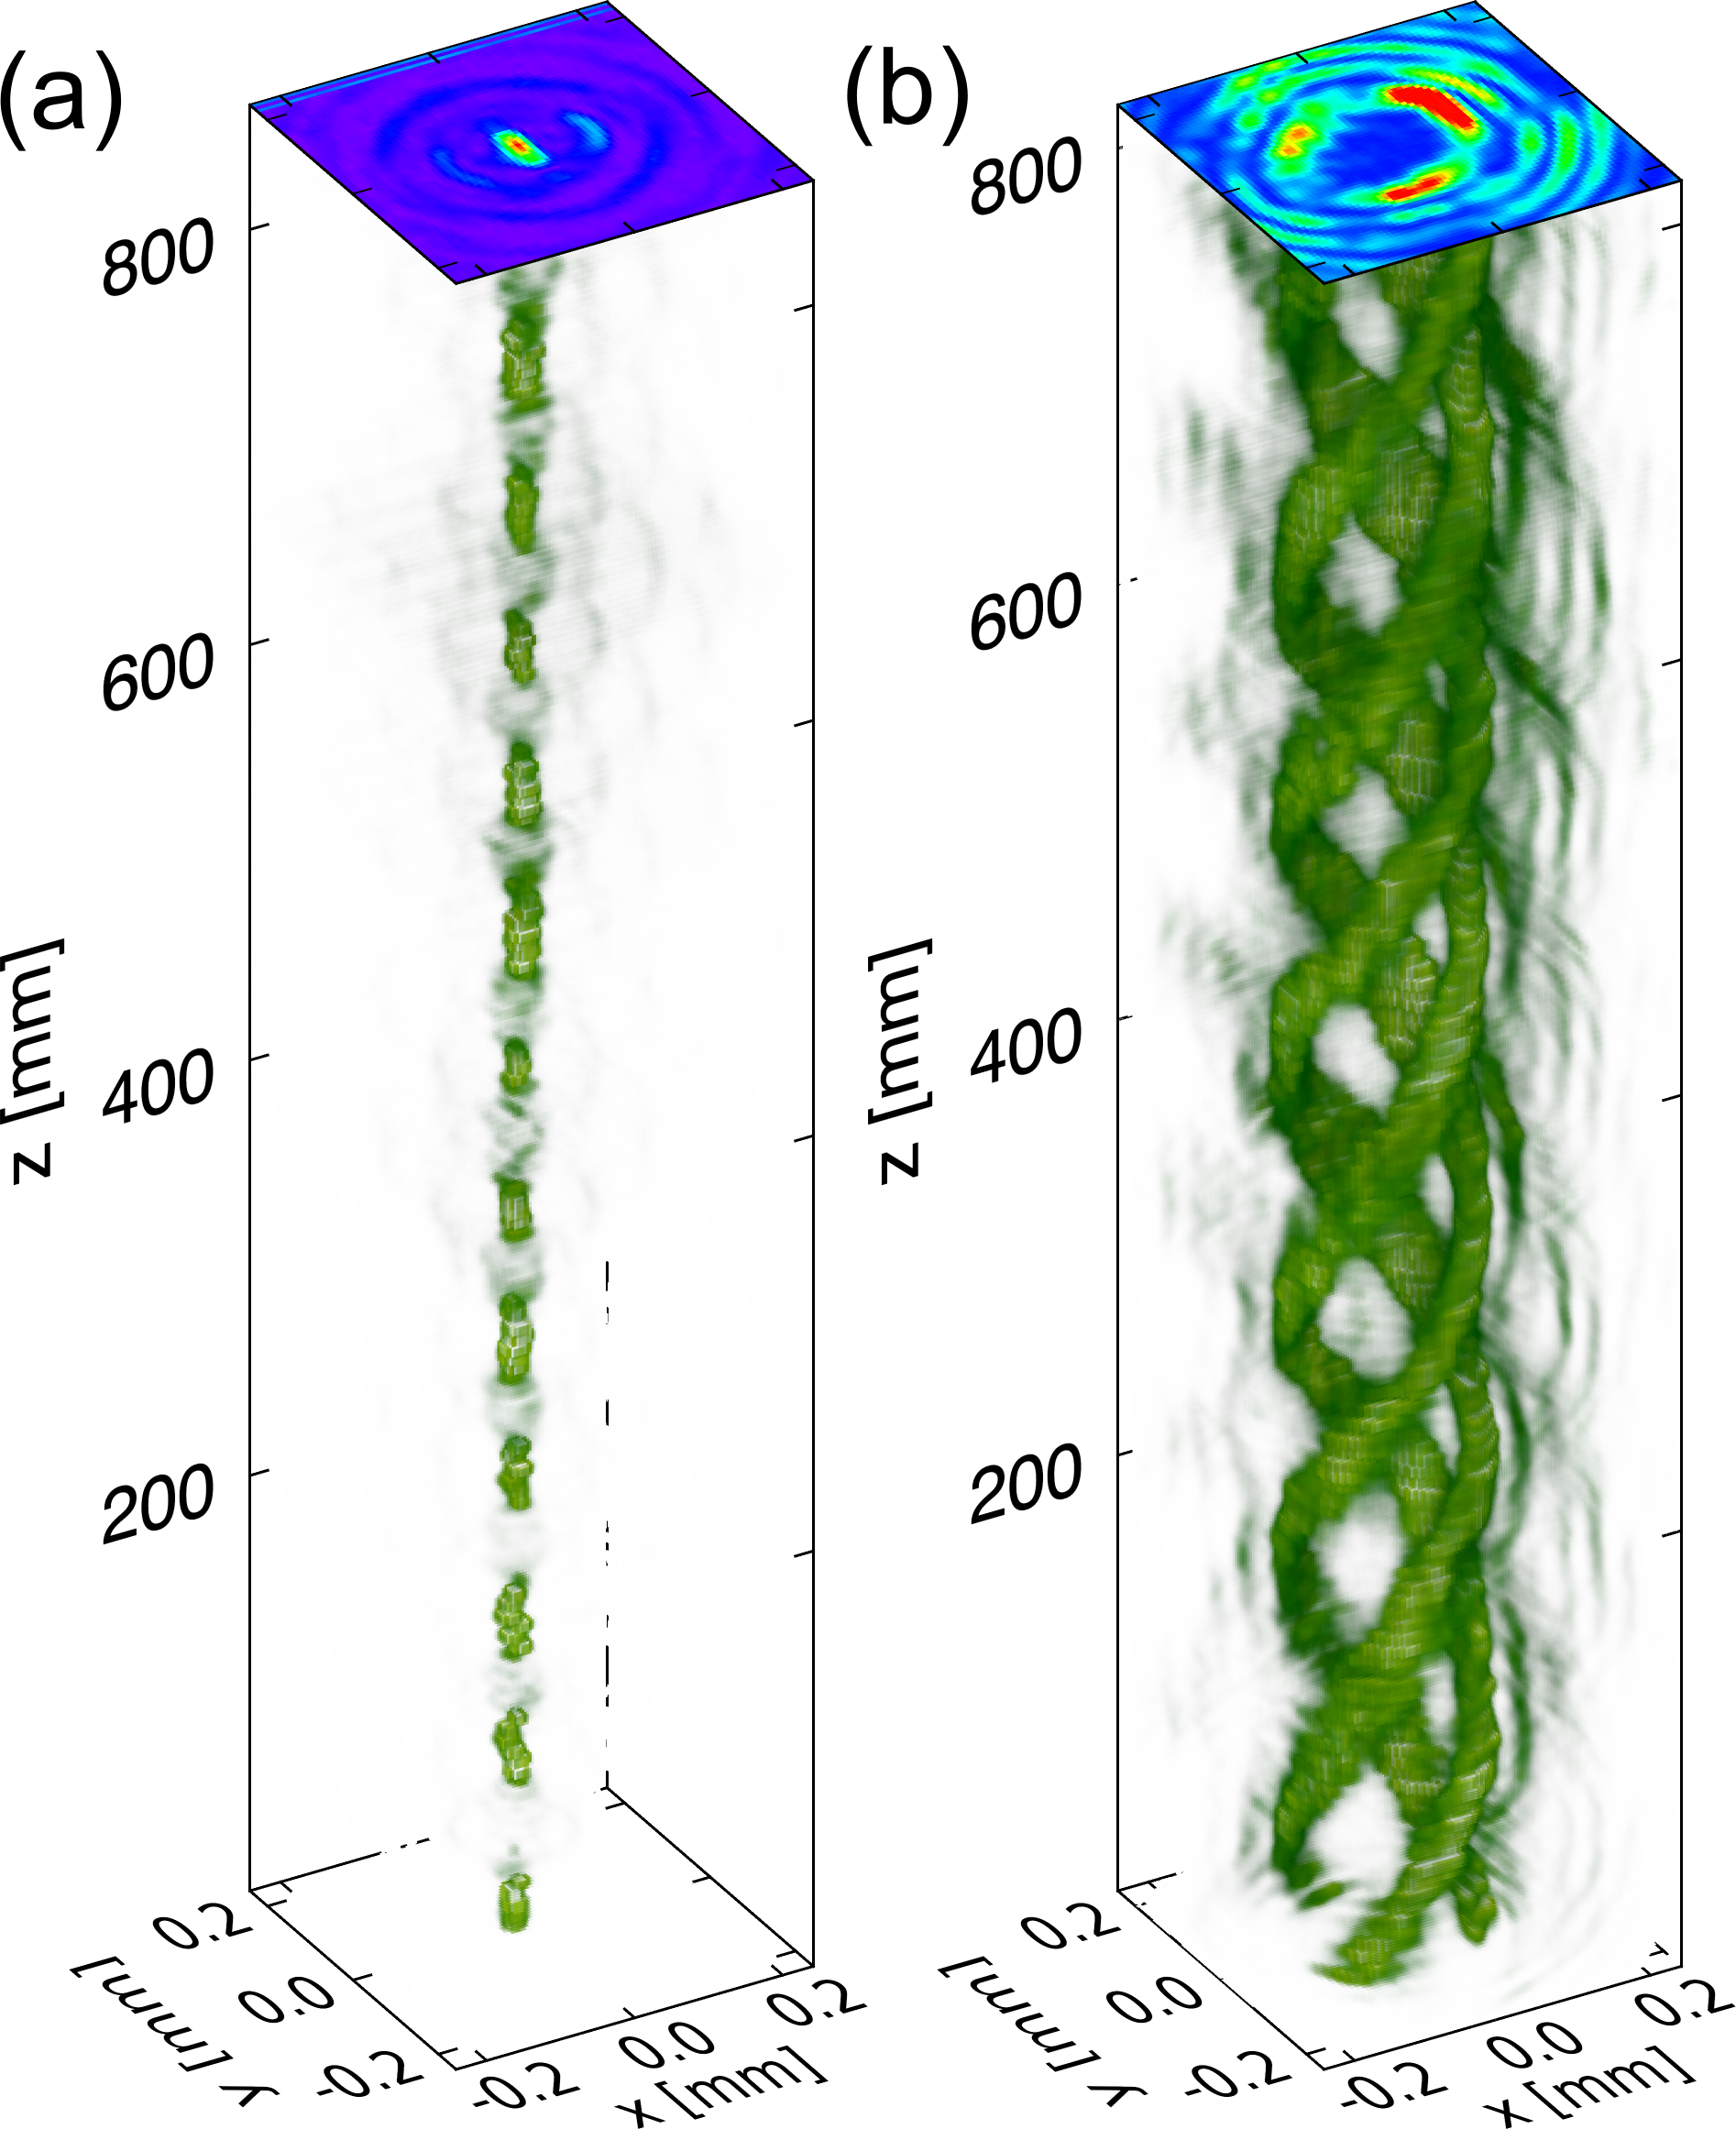
\includegraphics[width=0.75\columnwidth]{beams3}
  \caption{Tractor-beam modes projected with intermediate-plane
    holograms.}
  \label{fig:tractorbeams}
\end{figure}

Superpositions of Bessel beams can be obtained
by superposing results of the form predicted
by Eq.~\eqref{eq:besselfield} \cite{mcgloin03b}.
These are particularly useful for projecting
tractor beams.
The field for an optical conveyor
\cite{cizmar05,ruffner12a,ruffner14},
for example, can be as simple as a two-fold superposition
of equal-helicity Bessel beams:
\begin{equation}
  \label{eq:conveyorfield}
  E_{\alpha,m}^{\delta \alpha}(\vec{r},\phi)
  =
  E_{\alpha,m}(\vec{r})
  +
  e^{i \phi} \,
  E_{\alpha+\delta\alpha,m}(\vec{r}).
\end{equation}
An example with $m = 0$, $\alpha = \SI{5e-3}{\radian}$
and $\delta \alpha = \SI{1e-4}{\radian}$ % XXX check all numbers
is presented in Fig.~\ref{fig:tractorbeams}(a).
This linearly polarized beam was created at $\lambda = \SI{532}{\nm}$
(Coherent Verdi 5W)
using a phase-only spatial light modulator (SLM, Hamamatsu X10468-16)
to imprint the phase of the field described by
Eq.~\eqref{eq:conveyorfield}
on the collimated beam's wavefronts.
This beam's axial intensity profile is characterized by
a periodic array of maxima spaced by
$\Delta z = \lambda [\tan (\alpha + \delta\alpha) - \tan
\alpha]^{-1}$.
The alternating intensity maxima and minima act as
traps for illuminated objects that can be moved
along the beam's axis by
varying the relative phase, $\phi$
\cite{cizmar05,ruffner12a,ruffner14}.

The beam's intensity profile was measured by
moving a standard
video camera (NEC TI-324AII) along an optical rail in \SI{5}{\mm}
increments.
The resulting stack of transverse slices then was combined into
a volumetric data set with \SI{6.4}{\um} transverse spatial
resolution.
The transverse width of the intensity maxima does not change
appreciably over a range of \SI{2}{\meter}.
Figure~\ref{fig:tractorbeams}
is limited to a range of \SI{0.8}{\meter} for clarity.

Images were recorded with a total beam power of \SI{3}{\milli\watt},
as recorded by an optical power meter (Coherent Lasermate).
The upper limit of the conveyor beam's power, \SI{1}{\watt}, was
set by the \SI{3}{\watt} limit of the SLM, with a total diffraction
efficiency of \num{0.3} into the desired mode.
This represents a factor of \num{400} improvement of diffraction
efficiency relative to a standard ring hologram
\cite{ruffner12a,ruffner14}
given the SLM's \num{800 x 600} array of phase pixels.
The beam's non-diffracting range exceeds that of previously
reported holographically-projected conveyor modes
\cite{ruffner12a,ruffner14}
by a factor of more than \num{e3}.

Intermediate-plane holography particularly useful for projecting
more sophisticated superpositions of Bessel beams, such
as the solenoidal wave presented in Fig.~\ref{fig:tractorbeams}(b).
This two-beam superposition has the general form
\begin{equation}
  \label{eq:solenoid}
  E_{\alpha,m}^{\mu}(\vec{r})
  =
  E_{\alpha,m}(\vec{r})
  +
  \frac{J_m(j'_{m,2})}{J_{m'}(j'_{m',1})}
  E_{\alpha',m'}(\vec{r}),
\end{equation}
where $m' = m + \mu$,
$\alpha' = (j'_{m,2}/j'_{m',1}) \, \alpha$, and
$j'_{m,n}$ is the $n$-th zero of $J'_m(x)$.
The particular realization in Fig.~\ref{fig:tractorbeams}(b)
is a three-fold ($\mu = 3$) tractor-beam mode \cite{yevick16}
with $m = 10$ and $\alpha = \SI{e-3}{\radian}$.
These parameters satisfy the condition
$\cos(\alpha) > [m/(m + \mu)] \cos(\alpha + \delta \alpha)$
required for a solenoidal wave to act as a tractor beam
\cite{yevick16}. % XXX double check this.
As for the conveyor beam, the intermediate-plane hologram
projecting the solenoidal tractor beam has a diffraction
efficiency of roughly \num{0.3}, and yields a non-diffracting
range exceeding \SI{1}{\meter}.

Solenoidal modes are examples of accelerating waves \cite{berry79}
in the sense that the position of the principal intensity maximum,
is a non-linear function of axial position.
Intermediate-plane holography therefore is useful for creating
non-diffracting accelerating modes with high diffraction efficiency.

The same approach used for these demonstrations also can be
applied to more complicated superpositions of Bessel modes
\cite{cizmar09,vasilyeu09,lee10,litvin11}. % XXX related citations.
In all cases, the intermediate-plane approach should provide
better mode purity, longer range and higher diffraction efficiency
than conventional holographic mode-conversion techniques.

In addition to projecting collimated modes, intermediate-plane
holograms can project waves that converge or diverge at
a specified rate.  This is achieved by deliberately mis-matching
the placement of the intermediate plane with the back focal
plane of the converging element.  For intermediate-plane holograms
with integrated converging phase profiles, this is achieved by
having the displacement, $z$, differ from the focal length $f$.
In that case, the resulting divergence angle is
$\gamma = \tan^{-1}(1 - z/f)$. % XXX check sign
Each superposed mode in such an element, furthermore, can have
a different divergence angle.

Intermediate-plane holography is particularly useful for projecting
modes whose ideal Fresnel holograms are dominated by large
amplitude variations, and so suffer from low diffraction efficiency.
In addition to improving diffraction efficiency, shifting the
hologram plane also can improve mode purity by moving the
length scale for phase variations into the spatial bandwidth of a
practical diffractive optical element.
Both of these element figure in the success of intermediate-plane
holograms for projecting Bessel beams and their superpositions.
Because Bessel beams are the natural basis for propagation-invariant
modes, intermediate-plane holography lends itself naturally
to long-range projection.
We have demonstrated meter-scale projection using centimeter-scale
optical elements.
These same elements have additional potential applications for
topologically multiplexing and demultiplexing non-diffracting modes
for optical communications \cite{gibson04,bozinovic13,willner15}.
The same ability to project sophisticated superpositions of
topological modes could have additional applications to remote
sensing and LIDAR \cite{cvijetic15}.
Finally, the same principals discussed here in the context of
optical holography should apply equally well to other types
of waves, most notably to acoustic waves.

This work was supported primarily by the National Science Foundation
through Award no.\ DMR-1305875 and in part by NASA through
Award no.\ NNX13AK76G and through the NASA Space Technology Research
Fellowship (NSTRF) program under Award no.\ NN14AQ40H.

\bibliography{abbreviations,grier,dgg,tweezer}

\end{document}

%%% Local Variables:
%%% mode: latex
%%% TeX-master: t
%%% End:
